\chapter{Experimental Results}

All experiments in this thesis used a set of standard conditions.  First, the length and width of each puzzle piece was set to 28 pixels per the standard established by~\cite{cho2010} and subsequently used by~\cite{pomeranz2011, gallagher2012, sholomon2013, paikin2015}. What is more, the Mixed-Bag Solver was passed no information concerning piece location nor rotation.  Furthermore, no information concerning the size of the dimensions or number of pieces in each ground-truth image is provided to the solver.  Concerning the number of input puzzles, Paikin~\& Tal's algorithm requires this information; as such, all runs of their algorithm were supplied this, meaning their algorithm is by definition solving a simpler problem.  Despite that, the Mixed-Bag Solver still generally outperforms their algorithm.

\subsection{Single Puzzle Solving}

Pomeranz~\textit{et al.}~\cite{pomeranzBenchmarkImages} created an image dataset of 20~images that each contained 805 pieces.  This experiment serves to determine the baseline accuracy of the solver to predict the number of ground-truth inputs.  

The solver was able to identify that there was only a single puzzle in 17 out of the 20 images.  For remaining 3 images, the solver estimated that there were 2 images, meaning the margin of error was only a single puzzle.  Appendix~\ref{} shows the ground-truth image as well as the outputs from Paikin~\& Tal's algorithm as well as this thesis' Mixed-Bag Solver.  

The Mixed-Bag Solver struggled most with images where there are large areas with little variation (e.g., a blue sky, smooth water, etc.).  This is due to the fact that in such areas the Best Buddy Density is low; what is more, there are a significant number of interior non-adjacent internal best buddies.  Figure~\ref{fig:pomeranzBestBuddiesVisualizations} shows two images in the Pomeranz~\textit{et al.} dataset.  The Mixed-Bag Solver was able to perfectly reconstruct image (a); the Mixed-Bag Solver incorrectly determined found two separate images in (b) as shown in Appendix~\ref{}.  As the accompanying best buddy visualizations show, this error was caused by the fact that image (b) has far lower Best Buddy Density in the upper-left and lower right corner of the images.  What is more, image (b) also has significantly more interior non-adjacent best buddies. 

\begin{figure}[tb]
\centering
  \begin{tabular}{ >{\centering\arraybackslash}m{0.47\textwidth} >{\centering\arraybackslash}m{0.47\textwidth} }

	\fbox{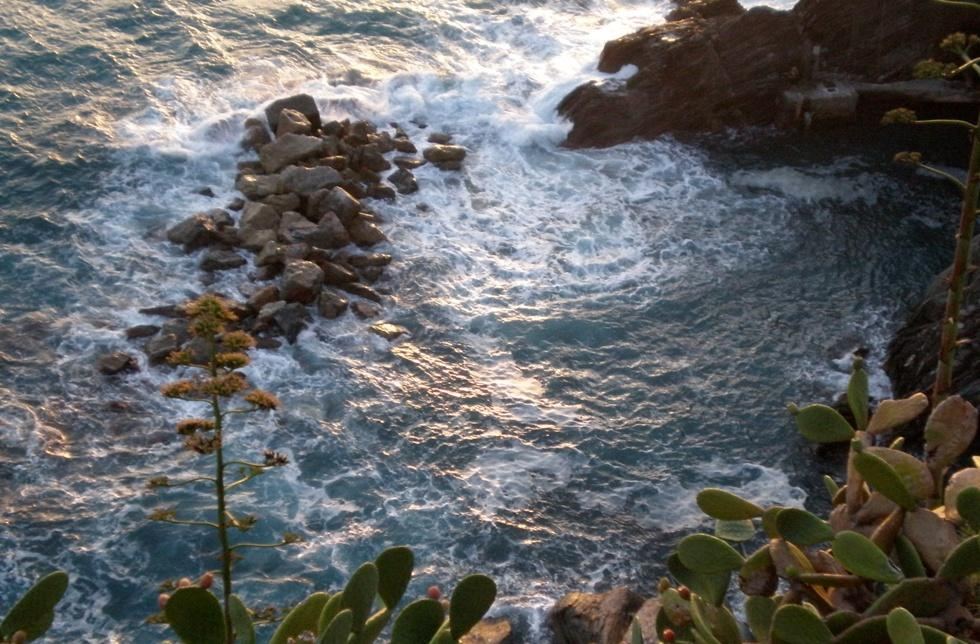
\includegraphics[scale=0.18]{./images/single_puzzle/pomeranz_805_14.jpg}} & \fbox{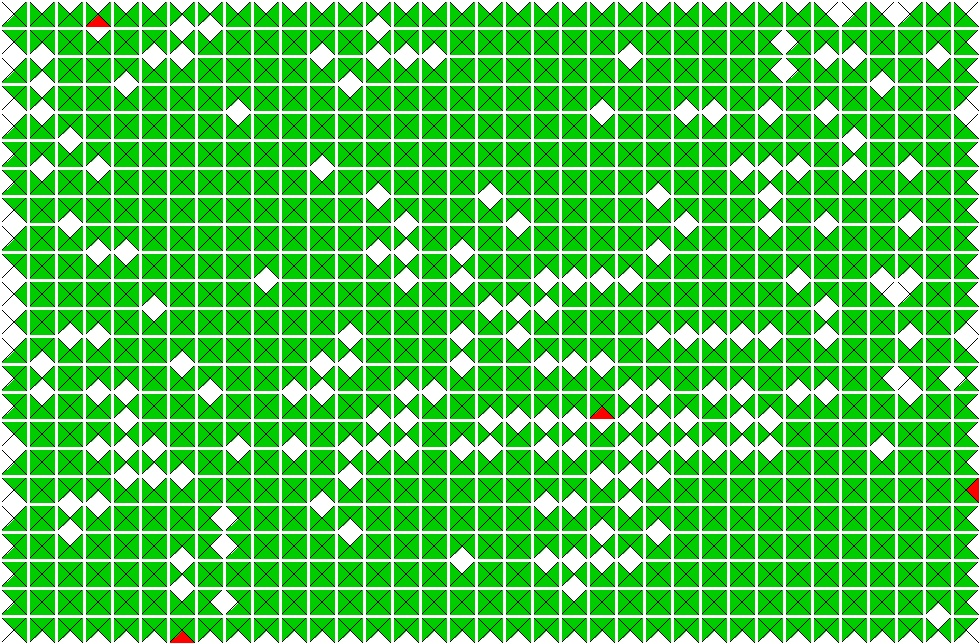
\includegraphics[scale=0.18]{./images/single_puzzle/best_buddies_pomeranz_805_14.jpg}} \\~\\
	Ground-Truth Image (a) & Best Buddy Visualization of Image (a) 
\\~\\
	\fbox{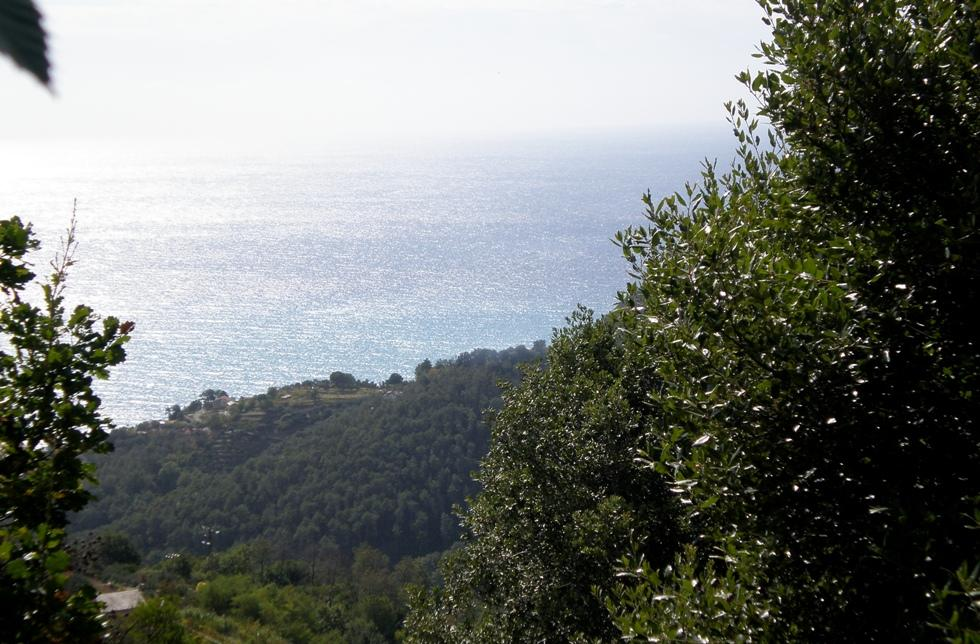
\includegraphics[scale=0.18]{./images/single_puzzle/pomeranz_805_12.jpg}} & \fbox{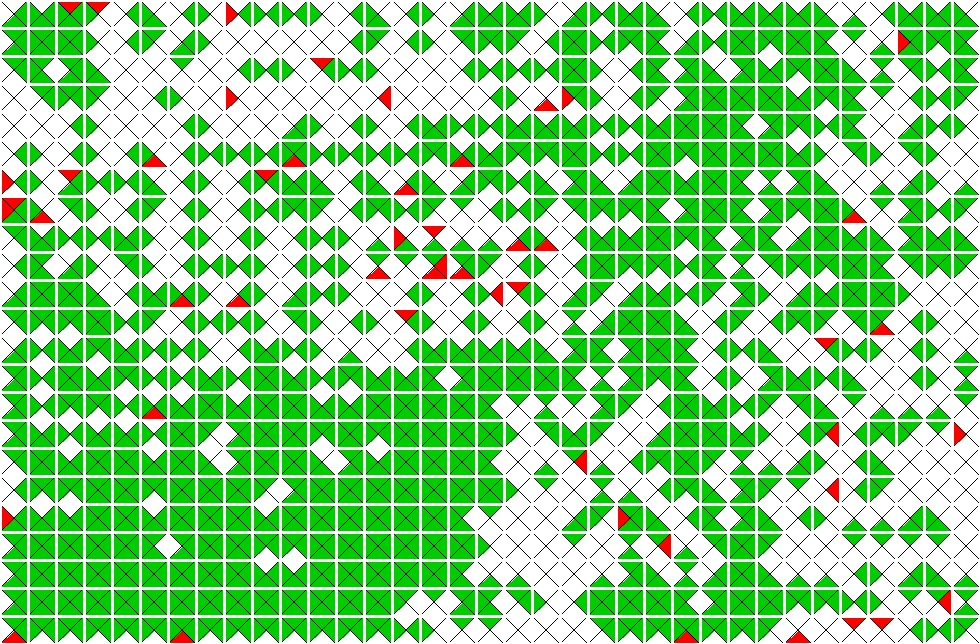
\includegraphics[scale=0.18]{./images/single_puzzle/best_buddies_pomeranz_805_12.jpg}} \\~\\
	Ground-Truth Image (b) & Best Buddy Visualization of Image (b) 
  \end{tabular}

\caption{Comparison of Best Buddy Density and Interior Non-Adjacent Best Buddies for Two Images from the Pomeranz \textit{et al.} 805 Piece Dataset}
\label{fig:pomeranzBestBuddiesVisualizations}
\end{figure} 

\subsection{Ten Puzzle Solving}

In the current literature, the most puzzles solved simultaneously by a Mixed-Bag Solver is five by \cite{paikin2015}; what is more, their solver received the number of input puzzles.  In contrast, this thesis has been shown to reconstruct ten puzzles of varying sizes.  Appendix~\ref{chap:tenPuzzleSolving} shows the input puzzles as well as the Mixed-Bag Solver outputs. When the identical set of puzzles were supplied to Paikin~\& Tal's algorithm, the seeds for nine of the puzzles came from just three of the input puzzles.  Table~\ref{}